% \begin{figure}[h]
% \centering
% \begin{tikzpicture}[scale=0.7]
%     % Red diagonal for first 3x3
%     \foreach \i in {1,2,3}
%     {
%         \fill[orange] (\i-1,6-\i) rectangle (\i,7-\i);
%     }
    
%     % Blue causal mask for second 3x3
%     \fill[cyan] (3,4) rectangle (4,5);
%     \fill[cyan] (3,3) rectangle (4,4);
%     \fill[cyan] (4,3) rectangle (5,4);

%     % ForestGreen causal mask for forth 3x3
%     \fill[ForestGreen] (3,0) rectangle (4,3);
%     \fill[ForestGreen] (4,0) rectangle (5,2);
%     \fill[ForestGreen] (5,0) rectangle (6,1);


%     % Grid
%     \draw[step=1cm,gray,very thin] (0,0) grid (6,6);

%     % Labels for columns (noisy sequences)
%     \foreach \x in {1,...,3}
%     {
%         \node[anchor=north] at (\x-0.5,-0.1) {$\mathbf{x}_t^{\x}$};
%     }

%     \foreach \x in {4,...,6}
%     {
%         \node[anchor=north] at (\x-0.5,-0.1) {$\mathbf{x}^{\x}$};
%     }
    
%     % Labels for rows (noisy sequences)
%     \foreach \y in {1,...,3}
%     {
%         \node[anchor=east] at (-0.1,6.5-\y) {$\mathbf{x}_t^{\y}$};
%     }

%     \foreach \y in {4,...,6}
%     {
%         \node[anchor=east] at (-0.1,6.5-\y) {$\mathbf{x}^{\y}$};
%     }
    
%     % Title
% \end{tikzpicture}
% \caption{Example of Specialized Attention Mask}
% \label{fig:attention_mask}
% \end{figure}

\definecolor{ForestGreen}{RGB}{34,139,34} % Forest green in RGB

\begin{figure}[h]
\centering
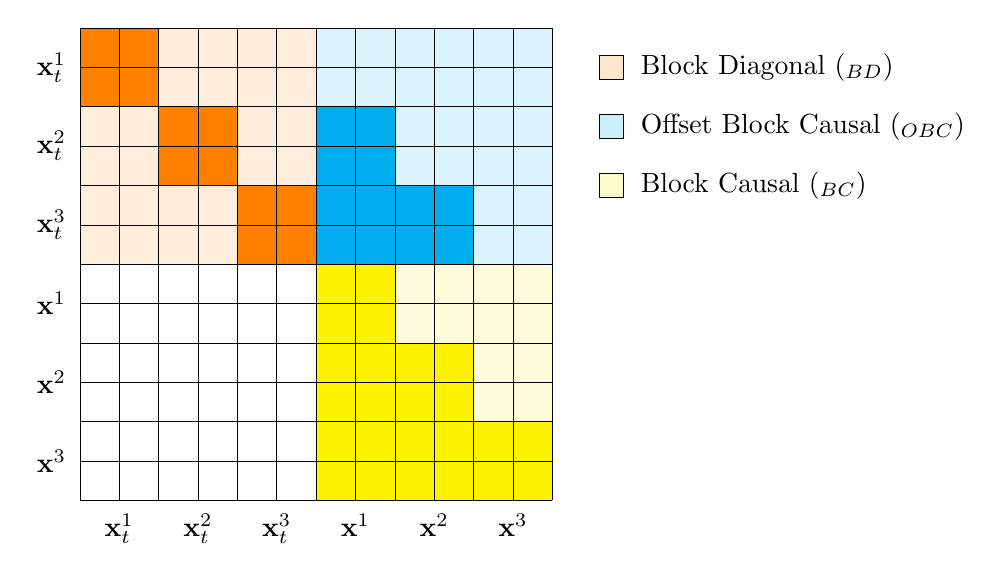
\begin{tikzpicture}[scale=0.5]
    % Grid
    % \draw[step=1cm,gray,very thin] (0,0) grid (12,12);

    % Block Diagonal
    \fill[orange!20, opacity=0.7] (0,12) rectangle (6,6);
    \foreach \i in {1,2,3}
    {
        \fill[orange] ({(\i-1)*2},{12-((\i-1)*2)}) rectangle ({(\i*2)},{12-(\i*2)});
    }

    % Block Causal Mask
    \fill[cyan!20, opacity=0.7] (6,12) rectangle (12,6);
    \fill[cyan] (6,10) rectangle (8,6);
    \fill[cyan] (8, 8) rectangle (10,6);

    % Block Causal for clean
    \fill[yellow!20, opacity=0.7] (6,6) rectangle (12,0);
    \fill[yellow] (6,6) rectangle (8,0);
    \fill[yellow] (8, 4) rectangle (10,0);
    \fill[yellow] (10, 2) rectangle (12,0);

    % Grid
    \draw[step=1cm,black,very thin] (0,0) grid (12,12);

    \foreach \x in {1, 3, 5}{
        \node[anchor=north] at (\x, -0.1) {$\mathbf{x}_t^{\pgfmathparse{int((\x/2)+1)}\pgfmathresult}$};
    }
    \foreach \x in {7, 9, 11}{
        \node[anchor=north] at (\x, -0.1) {$\mathbf{x}^{\pgfmathparse{int(((\x-6)/2)+1)}\pgfmathresult}$};
    }

    \foreach \y in {1, 3, 5}{
        \node[anchor=east] at (-0.1, 12-\y) {$\mathbf{x}_t^{\pgfmathparse{int((\y/2)+1)}\pgfmathresult}$};
    }
    \foreach \y in {7, 9, 11}{
        \node[anchor=east] at (-0.1, 12-\y) {$\mathbf{x}^{\pgfmathparse{int(((\y-6)/2)+1)}\pgfmathresult}$};
    }

    % Legend
    \node[draw, fill=orange!20, minimum width=0.3cm, minimum height=0.3cm] at (13.5, 11) {};
    \node[right] at (14, 11) {Block Diagonal ($\M_{BD}$)};
    
    \node[draw, fill=cyan!20, minimum width=0.3cm, minimum height=0.3cm] at (13.5, 9.5) {};
    \node[right] at (14, 9.5) {Offset Block Causal ($\M_{OBC}$)};
    
    \node[draw, fill=yellow!20, minimum width=0.3cm, minimum height=0.3cm] at (13.5, 8) {};
    \node[right] at (14, 8) {Block Causal ($\M_{BC}$)};

\end{tikzpicture}
\caption{Example of Specialized Attention Mask}
\label{fig:attention_mask_2}
\end{figure}


% \begin{python}

% # Define parameters
% seq_len = 128
% block_size = 16
% batch_size = 4
% num_heads = 8
% device = "cuda" if torch.cuda.is_available() else "cpu"

% # Create block mask
% my_block_diff_mask = partial(block_diff_mask, seq_len=seq_len, block_size=block_size)
% my_block_mask = create_block_mask(
%     my_block_diff_mask,
%     batch_size, num_heads, seq_len, seq_len, device=device, _compile=True
% )

% # **Single-Pass Flex Attention with Concatenated Sequence**
% @torch.compile(fullgraph=True, mode="max-autotune")
% def single_pass_block_diff_attn(q, k, v, block_mask):
%     return flex_attention(q, k, v, block_mask=block_mask)
% \end{python}



% \definecolor{ForestGreen}{RGB}{164,194,244}
% \definecolor{LightBlue}{RGB}{240,184,124}

% \begin{figure}[h]
% \centering
% \begin{tikzpicture}[scale=0.5]
%     % --- Colored Masks ---
%     % Draw each individual cell with white borders
%     \foreach \i in {0,...,5} {
%         \foreach \j in {0,...,5} {
%             \fill[white!20, draw=white] (\i,12-\j) rectangle (\i+1,11-\j);
%             \fill[white!20, draw=white] (\i+6,12-\j) rectangle (\i+7,11-\j);
%             \fill[white!20, draw=white] (\i+6,6-\j) rectangle (\i+7,5-\j);
%             \fill[white!20, draw=white] (\i,6-\j) rectangle (\i+1,5-\j);
%         }
%     }

%     % Block Diagonal (Upper-left)
%     \foreach \i in {1,2,3}{
%         \fill[LightBlue] ({(\i-1)*2},{12-((\i-1)*2)}) rectangle ({(\i*2)},{12-(\i*2)});
%     }

%     % Offset Block Causal (Upper-right)
%     \fill[ForestGreen] (6,10) rectangle (8,6);
%     \fill[ForestGreen] (8, 8) rectangle (10,6);

%     % Block Causal (Lower-right)
%     \fill[ForestGreen] (6,6) rectangle (8,0);
%     \fill[ForestGreen] (8, 4) rectangle (10,0);
%     \fill[ForestGreen] (10, 2) rectangle (12,0);


%     % Inner cell lines
%     \foreach \i in {1,...,5}{
%         \draw[white, thick] (\i,12) -- (\i,6);
%         \draw[white, thick] (\i+6,12) -- (\i+6,6);
%         \draw[white, thick] (\i,6) -- (\i,0);
%         \draw[white, thick] (\i+6,6) -- (\i+6,0);
%         \draw[white, thick] (0,12-\i) -- (6,12-\i);
%         \draw[white, thick] (6,12-\i) -- (12,12-\i);
%         \draw[white, thick] (0,6-\i) -- (6,6-\i);
%         \draw[white, thick] (6,6-\i) -- (12,6-\i);
%     }

%         % --- Quadrant Bounding Boxes ---
%     \draw[thick, black] (0,12) rectangle (6,6);    % Upper-left
%     \draw[thick, black] (6,12) rectangle (12,6);   % Upper-right
%     \draw[thick, black] (0,6) rectangle (6,0);     % Lower-left
%     \draw[thick, black] (6,6) rectangle (12,0);    % Lower-right


%     % Axis labels
%     \foreach \x in {1, 3, 5}{
%         \node[anchor=north] at (\x, -0.1) {$\mathbf{x}_t^{\pgfmathparse{int((\x/2)+1)}\pgfmathresult}$};
%     }
%     \foreach \x in {7, 9, 11}{
%         \node[anchor=north] at (\x, -0.1) {$\mathbf{x}^{\pgfmathparse{int(((\x-6)/2)+1)}\pgfmathresult}$};
%     }

%     \foreach \y in {1, 3, 5}{
%         \node[anchor=east] at (-0.1, 12-\y) {$\mathbf{x}_t^{\pgfmathparse{int((\y/2)+1)}\pgfmathresult}$};
%     }
%     \foreach \y in {7, 9, 11}{
%         \node[anchor=east] at (-0.1, 12-\y) {$\mathbf{x}^{\pgfmathparse{int(((\y-6)/2)+1)}\pgfmathresult}$};
%     }

% \end{tikzpicture}
% \caption{Example of Specialized Attention Mask with White Borders}
% \label{fig:attention_mask_quadrants_white}
% \end{figure}



